
\documentclass[aspectratio=169]{beamer}
\usepackage[utf8]{inputenc}
\usepackage[T1]{fontenc}
\usepackage[french]{babel}
\usepackage{amsmath}
\usepackage{booktabs}
\usepackage{graphicx}
\usetheme{Madrid}
\usecolortheme{default}
\title{Projet de Recherche Opérationnelle}
\subtitle{Routage, affectation, EOQ et méthode du simplexe}
\author[C25936 -- C30620]{Réalisé par :\\C25936 -- MOHAMED CHERIV\\C30620 -- MOHAMEDEN ELBEDEWI}
\date{Année universitaire 2025--2026}

\begin{document}

\begin{frame}
\titlepage
\end{frame}

\begin{frame}{Plan de la présentation}
\begin{enumerate}
\item Outils recommandés utilisés
\item Routage des camions d'eau
\item Affectation des étudiants aux projets
\item Dimensionnement de stock EOQ
\item Méthode du simplexe
\item Comparaison et conclusion
\end{enumerate}
\end{frame}

\begin{frame}{Objectif général}
\begin{itemize}
\item Appliquer la recherche opérationnelle à plusieurs problèmes pratiques.
\item Modéliser les décisions avec variables, objectifs et contraintes.
\item Interpréter les résultats obtenus par calcul ou algorithme.
\end{itemize}
\end{frame}

\begin{frame}{1. Routage des camions d'eau}
\begin{columns}
\column{0.52\textwidth}
\begin{itemize}
\item Problème réel en Mauritanie.
\item 1 dépôt central.
\item 6 points de distribution.
\item Capacité du camion : 1000 L.
\item Objectif : minimiser la distance totale.
\item Outil : Python + NetworkX.
\end{itemize}
\column{0.48\textwidth}
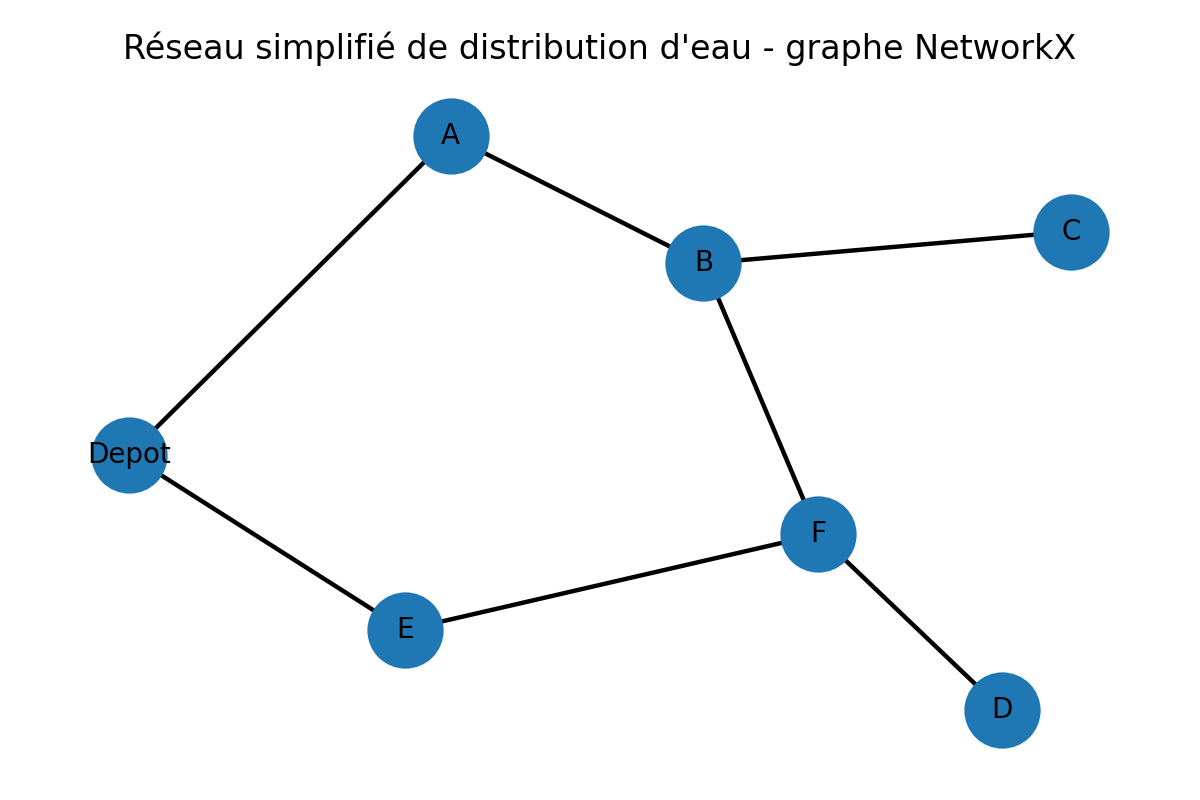
\includegraphics[width=\textwidth]{figures/water_network.png}
\end{columns}
\end{frame}

\begin{frame}{Modèle de routage}
\[
\min Z = \sum d_{ij}x_{ij}
\]
\begin{itemize}
\item $d_{ij}$ : distance entre deux points.
\item $x_{ij}=1$ si le camion va de $i$ vers $j$.
\item Chaque point doit être visité.
\item La capacité du camion ne doit pas être dépassée.
\item Le réseau est représenté par un graphe pondéré NetworkX.
\end{itemize}
\end{frame}

\begin{frame}{Méthode utilisée pour le routage}
\textbf{Heuristique du plus proche voisin}
\begin{enumerate}
\item Le camion part du dépôt.
\item Il choisit le point non visité le plus proche.
\item Il continue tant que la capacité restante le permet.
\item Il retourne au dépôt si la capacité devient insuffisante.
\end{enumerate}
\end{frame}

\begin{frame}{2. Affectation des étudiants aux projets}
\begin{columns}
\column{0.52\textwidth}
\begin{itemize}
\item 6 étudiants.
\item 3 projets.
\item Capacité : 2 étudiants par projet.
\item Objectif : maximiser la satisfaction totale.
\end{itemize}
\column{0.48\textwidth}
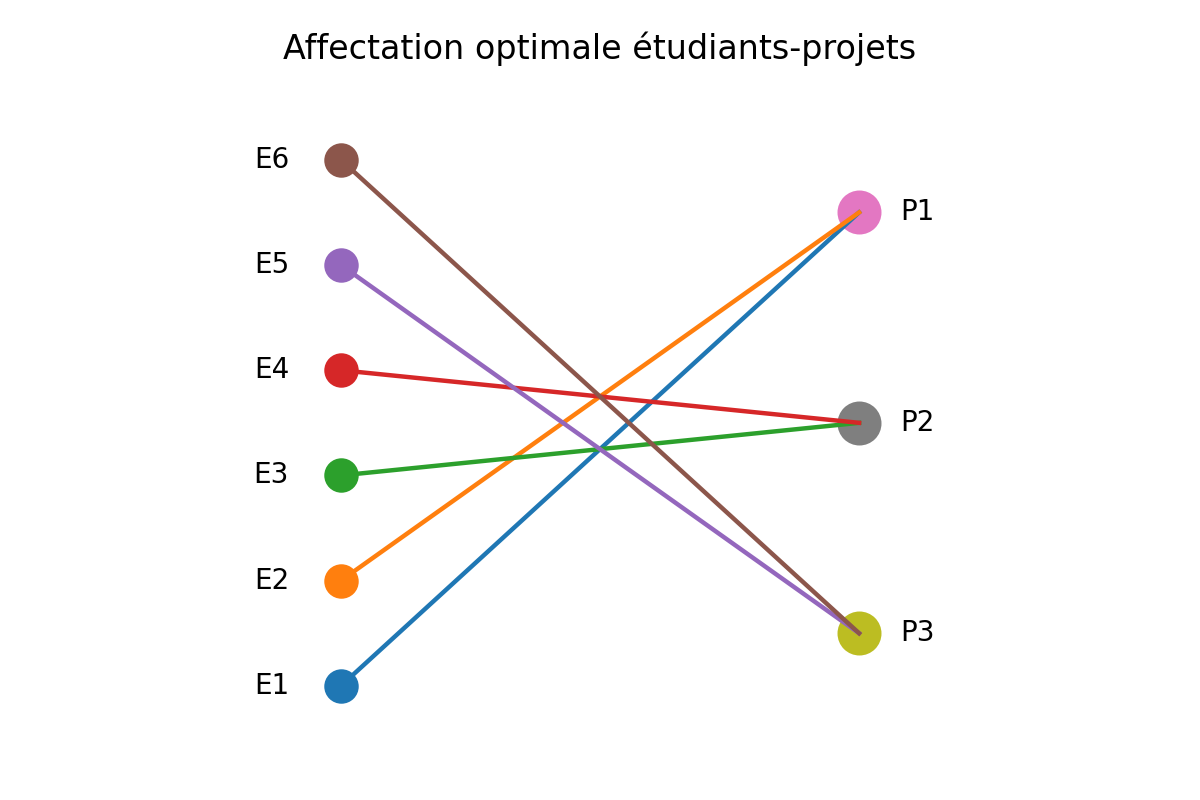
\includegraphics[width=\textwidth]{figures/student_assignment.png}
\end{columns}
\end{frame}

\begin{frame}{Modèle d'affectation}
\[
x_{ij}=\begin{cases}
1 & \text{si l'étudiant } i \text{ est affecté au projet } j \\
0 & \text{sinon}
\end{cases}
\]
\[
\max Z = \sum_{i=1}^{6}\sum_{j=1}^{3}p_{ij}x_{ij}
\]
\[
\sum_{j=1}^{3}x_{ij}=1,\quad \sum_{i=1}^{6}x_{ij}=2
\]
\end{frame}

\begin{frame}{3. Dimensionnement de stock EOQ}
\begin{columns}
\column{0.52\textwidth}
\begin{itemize}
\item Demande annuelle : $D=1200$.
\item Coût de commande : $S=50$ MRU.
\item Coût de stockage : $H=2$ MRU/unité/an.
\item Objectif : minimiser le coût total.
\end{itemize}
\column{0.48\textwidth}
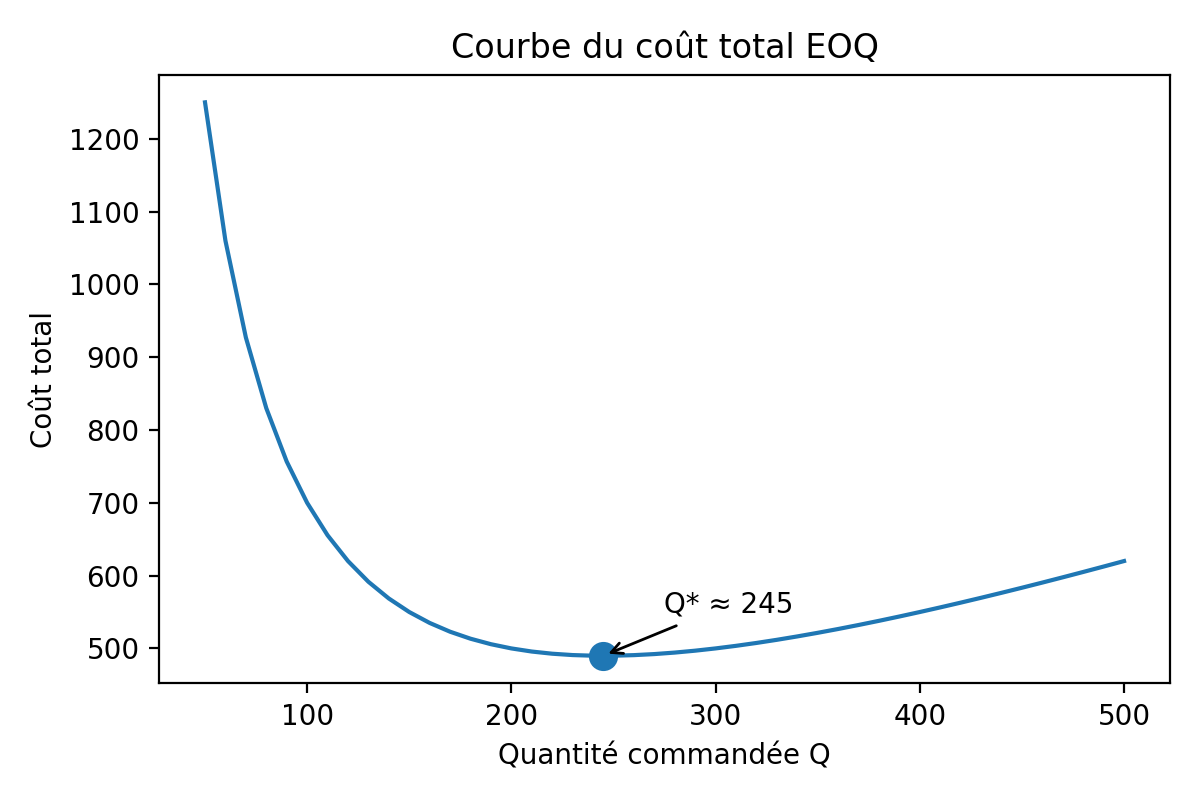
\includegraphics[width=\textwidth]{figures/eoq_curve.png}
\end{columns}
\end{frame}

\begin{frame}{Résultat EOQ}
\[
Q^* = \sqrt{\frac{2DS}{H}}
\]
\[
Q^* = \sqrt{\frac{2\times 1200\times 50}{2}} \approx 245
\]
\begin{block}{Interprétation}
La quantité économique de commande est d'environ 245 unités par commande.
\end{block}
\end{frame}

\begin{frame}{4. Méthode du simplexe}
\begin{columns}
\column{0.50\textwidth}
\[
\max z = 3x+4y
\]
\[
x+2y\leq 8
\]
\[
3x+y\leq 9
\]
\[
x,y\geq 0
\]
\column{0.50\textwidth}
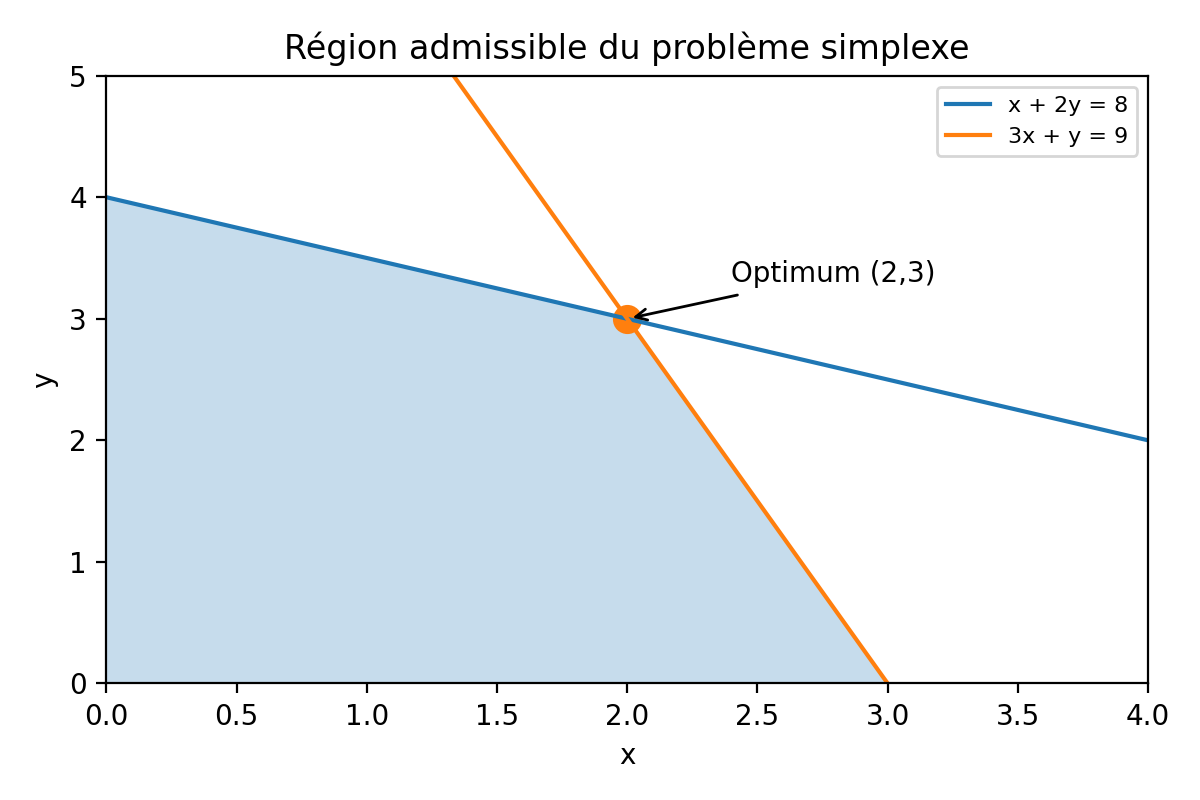
\includegraphics[width=\textwidth]{figures/simplex_region.png}
\end{columns}
\end{frame}

\begin{frame}{Tableau initial du simplexe}
\begin{center}
\begin{tabular}{c|ccccc}
\toprule
Base & $x$ & $y$ & $s_1$ & $s_2$ & RHS \\
\midrule
$s_1$ & 1 & 2 & 1 & 0 & 8 \\
$s_2$ & 3 & 1 & 0 & 1 & 9 \\
$z$ & -3 & -4 & 0 & 0 & 0 \\
\bottomrule
\end{tabular}
\end{center}
\begin{itemize}
\item Variable entrante initiale : $y$.
\item Les pivots conduisent à la solution optimale.
\end{itemize}
\end{frame}

\begin{frame}{Solution optimale par simplexe}
\[
x^*=2,\quad y^*=3
\]
\[
z^*=3(2)+4(3)=18
\]
\begin{block}{Interprétation}
La solution optimale utilise totalement les deux ressources :
$x+2y=8$ et $3x+y=9$.
\end{block}
\end{frame}

\begin{frame}{Comparaison des modèles}
\begin{tabular}{p{3.5cm}p{4.1cm}p{3.8cm}}
\toprule
Sujet & Type & Méthode \\
\midrule
Routage d'eau & VRP simplifié & NetworkX + plus proche voisin \\
Affectation & Optimisation binaire & Recherche exhaustive \\
EOQ & Stock & Formule analytique \\
Simplexe & PL & Pivots successifs \\
\bottomrule
\end{tabular}
\end{frame}

\begin{frame}{Conclusion}
\begin{itemize}
\item Le routage réduit les distances de livraison.
\item L'affectation maximise la satisfaction des étudiants.
\item EOQ minimise le coût de stock.
\item Le simplexe donne une solution optimale pour un programme linéaire.
\end{itemize}
\vspace{0.3cm}
\textbf{Conclusion :} la recherche opérationnelle aide à prendre de meilleures décisions avec des ressources limitées.
\end{frame}

\end{document}
